\section{Introduction}
\label{sec:intro}

\begin{figure}[!th]
    \centering
    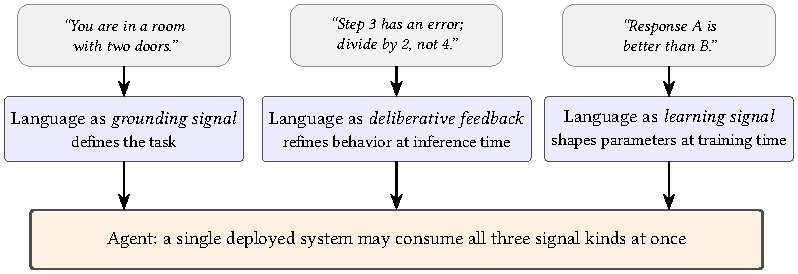
\includegraphics[width=\linewidth]{paper_images/generated/overview.pdf}
    \Description{Three example language signals map to grounding, deliberative feedback, and learning. Arrows from all three roles point to one agent, showing that a single system may consume the roles together.}
    \caption{Language plays three complementary roles as a signal in agentic systems: grounding the task and environment, scaffolding intermediate deliberation, and serving as a learning signal for training. The three roles classify signals, not system stages; a single deployed system may consume all three (\S\ref{sec:taxonomy}).}
    \label{fig:overview}
\end{figure}

Classical reinforcement learning assumes a specified environment, action space, and reward. Its landmark successes therefore depend on substantial domain engineering and on objectives whose optima match their designers' intent \citep{mnih2015human,silver2016mastering,vamplew2021scalarrewardenoughresponse}. This specification burden is most acute for ambiguous, context-dependent tasks that resist scalar rewards \citep{amodei2016concrete}.

Large language models open a second supervisory channel: language can express task intent, diagnose an output, preserve a lesson, or supply training feedback in a form an agent can consume directly \citep{brown2020language,achiam2023gpt,madaan2023selfrefine}. The central question is no longer only how to derive a better scalar reward, but when retaining the structure of a critique, rubric, or instruction changes what can be learned.

We call the resulting family \textbf{verbal reinforcement learning (VRL)} and impose two membership criteria. First, feedback is expressed in natural language and its linguistic structure is functionally consumed, rather than collapsed to a scalar or preference bit before use. Second, it participates in an improvement loop through output revision, memory write, parameter update, or construction of a decision-problem component that later drives such an update. Both criteria are required. Plain instruction following fails the second. Vanilla RLHF \citep{christiano2017deep,ouyang2022training} and DPO \citep{rafailov2023direct} fail the first because the rationale is discarded before learning. Language-conditioned RL treats language as policy input while an ordinary scalar reward drives improvement. Reward-code generation remains inside the fence because a compiler consumes the language before the resulting reward drives optimization. Only feedback must be textual, so agents with visual observations remain in scope when their corrections are verbal (\S\ref{sec:embodied}). Section~\ref{sec:framework} formalizes this fence.

We organize qualifying signals by when they take effect and what they modify. A \emph{grounding signal} defines goals, states, actions, or reward structure at problem-definition time. \emph{Deliberative feedback} revises context, output, or memory during inference without changing weights. A \emph{learning signal} changes parameters or training data. These are roles of signals, not mutually exclusive system types or lifecycle stages: one agent can consume all three. Existing surveys usually organize by correction mechanism, agent component, or optimization family \citep{pan2023automatically,zhang2025survey,wang2024reinforcement}; our signal-centric axis instead connects problem definition, inference, training, credit assignment, evaluation, and feedback-channel safety.

This article makes four contributions.
\begin{enumerate}
    \item \textbf{Formalism and taxonomy.} A language-augmented decision framework locates linguistic artifacts at six entry points, while an explicit assignment rule resolves hybrid methods by the component modified when a signal takes effect (\S\ref{sec:framework}, \S\ref{sec:taxonomy}).
    \item \textbf{Mechanism synthesis.} We connect the three pillars to the verbal reward stack, credit assignment, and language-space optimization, distinguishing outcome, process, token, context, memory, and parameter updates (\S\ref{sec:rewardstack}, \S\ref{sec:credit}, \S\ref{sec:optimizers}).
    \item \textbf{Evaluation and safety.} We separate feedback quality from feedback utilization and analyze attacks and defenses at the feedback channel rather than treating the signal as trusted input (\S\ref{sec:evaluation}, \S\ref{sec:safety}).
    \item \textbf{Practice and positioning.} We provide mechanism-selection rules, compare eighteen neighboring surveys and frameworks on fixed dimensions, and derive a focused research agenda (\S\ref{sec:practitioner}).
\end{enumerate}

Sections~\ref{sec:framework} and~\ref{sec:taxonomy} establish the formalism and taxonomy; Sections~\ref{sec:grounding} through~\ref{sec:learning} develop the pillars. The remaining sections treat rewards, credit, optimization, embodiment, evaluation, safety, and practitioner decisions before Section~\ref{sec:conclusion} concludes.
